\PassOptionsToPackage{table}{xcolor}
\documentclass[nobib,nofonts]{tufte-handout}

%\geometry{showframe} % display margins for debugging page layout

%%% MF additions
% \usepackage[table]{xcolor}
\usepackage[nographicx, nohyperref, nosubcaption, nogb4e, nobiblatex]{../99-auxiliary-files/00-mypackages}
\usepackage{../99-auxiliary-files/00-mycommands}
\usepackage{../99-auxiliary-files/00-myenvironments}

\usepackage{titlesec}
\usepackage{etoolbox}
\usepackage{tikz-qtree}
\usepackage{subcaption}

% \titleformat{\section}
% {\large\bfshape}{\thesection}{1em}{}

\setcounter{secnumdepth}{5}
\renewcommand\thesection{\arabic{section}}

% this length controls tha hanging indent for titles
% change the value according to your needs
\newlength\titleindent
\setlength\titleindent{0.7cm}

\pretocmd{\paragraph}{\stepcounter{subsection}}{}{}
\pretocmd{\subparagraph}{\stepcounter{subsubsection}}{}{}

\titleformat{\chapter}[block]
  {\normalfont\huge\bfseries}{}{0pt}{\hspace*{-\titleindent}}

\titleformat{\section}
  {\normalfont\Large\itshape}{\llap{\parbox{\titleindent}{\thesection\hfill}}}{0em}{}

\titleformat{\subsection}
  {\normalfont\itshape}{\llap{\parbox{\titleindent}{\thesubsection\hfill}}}{0em}{}

\titleformat{\subsubsection}
  {\normalfont\normalsize\itshape}{\llap{\parbox{\titleindent}{\thesubsubsection}}}{0em}{}

\titleformat{\paragraph}[runin]
  {\normalfont\normalsize\itshape}{}{-0.7cm}{}[\xspace \ \ \ \ ]

\titleformat{\subparagraph}[runin]
  {\normalfont\normalsize}{\llap{\parbox{\titleindent}{\thesubsubsection\hfill}}}{0em}{}

\titlespacing*{\chapter}{0pt}{0pt}{20pt}
\titlespacing*{\subsubsection}{0pt}{3.25ex plus 1ex minus .2ex}{1.5ex plus .2ex}
\titlespacing*{\paragraph}{0pt}{3.25ex plus 1ex minus .2ex}{0em}
\titlespacing*{\subparagraph}{0pt}{3.25ex plus 1ex minus .2ex}{0em}

\DefineNamedColor{named}{mygray2}{cmyk}{0.55,0.25,0.25,0.25}
\newcommand{\mygray}[1]{\textcolor{mygray2}{#1}}

%%% Tufte style
\usepackage{graphicx} % allow embedded images
  \setkeys{Gin}{width=\linewidth,totalheight=\textheight,keepaspectratio}
  \graphicspath{{graphics/}} % set of paths to search for images

\usepackage{fancyvrb} % extended verbatim environments
  \fvset{fontsize=\normalsize}% default font size for fancy-verbatim environments

% Standardize command font styles and environments
\newcommand{\doccmd}[1]{\texttt{\textbackslash#1}}% command name -- adds backslash automatically
\newcommand{\docopt}[1]{\ensuremath{\langle}\textrm{\textit{#1}}\ensuremath{\rangle}}% optional command argument
\newcommand{\docarg}[1]{\textrm{\textit{#1}}}% (required) command argument
\newcommand{\docenv}[1]{\textsf{#1}}% environment name
\newcommand{\docpkg}[1]{\texttt{#1}}% package name
\newcommand{\doccls}[1]{\texttt{#1}}% document class name
\newcommand{\docclsopt}[1]{\texttt{#1}}% document class option name
\newenvironment{docspec}{\begin{quote}\noindent}{\end{quote}}% command specification environment

\newcommand{\proplog}{\acro{PropLog}}
\newcommand{\predlog}{\acro{PredLog}}
\newcommand{\EFSQ}{\ensuremath{\mathit{EFSQ}}\xspace}

%%%%%%%%%%%%%%%%%%%%%%%%%%%%%%%%%%%%%%%%%%%%%%%%%%

% \usepackage[sc,osf]{mathpazo}
% \linespread{1.05}



\title{Predicate Logic}

\author[M.~Franke]{Michael Franke}

\date{} % without \date command, current date is supplied

\begin{document}

\maketitle

\begin{abstract}
\noindent
Formulas of predicate logic;
predicate letters, variables \& individual constants;
domain of quantification;
quantifier scope and binding;
atomic sentences;
predicate-logical meaning of natural language sentences;
semantics of predicate logic;
model, domain and interpretation function;
assignment and valuation functions;
validity;
predicate logic with identity
\end{abstract}

\section{Motivation}

We can think of propositional logic as a system that formalizes the meaning of important functional terms, namely the sentential connectives (negation, conjunction, disjunction, implication).
This carries a long way towards capturing what sound logical inference is.
But it also fails to capture crucial patterns of inference.
For example, if we know that
\begin{quote}
  Alex is as tall as Bo
\end{quote}
we also know that
\begin{quote}
  Bo is as tall as Alex
\end{quote}
in virtue of our knowledge of what the predicate ``being as tall as'' means.
Propositional logic cannot capture this.
It can model the first sentences as $p$ (= ``Alex is as tall as Bo'') and the second as $q$ (= ``Bo is as tall as Alex''), but since we cannot look inside the structure of a simple proposition, there is no way in which we can say that $p$, based on its internal form and relatedness to the internal form of $q$, must necessarily entail $q$.\sidenote{We can, of course, make the additional premise by writing down that $p \rightarrow q$, but that clearly does not explain the general relationship.}

Predicate logic (\predlog) is an extension of \proplog which adds two things.
Firstly, \predlog models the internal structure of atomic propositions in terms of \emph{predicates} and \emph{individual constants}.
For example, we could have a (two-place) predicate $T$ meaning (``being as tall as'') and two symbols, so-called individual constants, $a$ and $b$ which represent Alex and Bo respectively.
We can then translate the sentence ``Alex is as tall as Bo'' into the formula $Tab$, which is a minimal truth-evaluable unit, but does have internal structure.
Similarly, the sentence ``Bo is as tall as Alex'' would translate into $Tba$.

Secondly, \predlog allows to express \emph{quantification}, which is extremely important in order to represent general rules, generalizations and key aspects of our semantic and world knowledge.\sidenote{Semantic knowledge is what we know about the meaning of words and expressions. For example, semantic knowledge tells us that ``being taller than'' is a transitive relation, and that ``being as tall as'' is an equivalence relation. World knowledge is what we know about the world. For example, we know that Berlin is the capital of Germany.}
Imagine that you have a reasoning machine (computer, robot, friend \dots) able to compute logical inferences in predicate logic.
Even though we have not introduced any of the formal machinery (syntax, semantics, definition of validity, deduction system) necessary to make such formal reasoning precise, imagine you give this machine the information $Tab$.
You want it to represent ``Alex is as tall as Bo,'' but the machine only has the string of symbols to work with.
Would that machine be able to conclude that $Tba$?
No, it wouldn't because it doesn't know that you want the symbol $T$ to mean ``being as tall as'' and not ``being taller than'' or anything else.
But, using predicate logic, you \emph{can} tell the system about the fundamental structural properties of the relation ``being as tall as,'' such as that it is reflexive.
In other words, you can express that ``being as tall as'' is a symmetric predicate in with the \predlog formula:
\begin{align*}
 \forall x \myts \forall y \myts (Txy \rightarrow Tyx)
\end{align*}
which can be read as ``for all objects $x$ and $y$, if $x$ stands in relation $T$ to $y$, then so does $y$ to $x$.''
This formula uses the quantifier \(\forall\) to express a generalization: something that holds of any pair of objects.
Generalizations of this kind are essential for human reasoning and \predlog captures the most basic aspects of quantification in a system of logical reasoning.
To be clear, the inference schema:
\begin{align*}
 Tab, \forall x \myts \forall y \myts (Txy \rightarrow Tyx) / Tba
\end{align*}
is logically valid in \predlog, but the schema:
\begin{align*}
 Tab / Tba
\end{align*}
is not.

\section{The language of predicate logic}

\subsection{Basic ingredients of predicate-logical formulas}

The formulas of \predlog consist:
\begin{multicols}{2}
\begin{itemize}
  \item individual constants $a,b,c, \dots, v$
  \item predicate letters $A, B, C, D \dots$
  \item variables $w, x,y,z$
  \item parentheses ( \ \ )
  \item sentential connectives $\neg, \wedge, \vee, \rightarrow, \leftrightarrow$
  \item quantifiers $\exists, \forall$
\end{itemize}
\end{multicols}
\emph{Individual constants} are denoted by lower-case Roman letters ($a, b, c, \dots, v $) up to $v$.\sidenote{If need be, we can also use indices like $a_{1}$, $a_{2}$ etc. This also holds for variables and predicate letters.}
Individual constants are like proper names: they refer to exactly one individual.
For example, the individual constant $a$ may be interpreted as referring to Alex and $b$ as referring to Bo.
Individuals in the sense of predicate logic need not be humans or animals. An individual is any kind of entity that can have properties or stand in some kind of relation to any other property. For example, constant $m$ may denote a particular copy of \emph{Moby Dick}.

\emph{Predicate letters} are denoted with upper-case Roman letters ($A, B, C, D \dots$).
Predicate letters will be used to denote properties or relations.
Each predicate letter has a unique \emph{arity}.
The arity of a predicate letter is always an integer bigger than zero.
It gives the number of elements that the predicate letter expects as an argument.
A predicate letter with arity one is also called \emph{unary} predicate letter and will be interpreted to refer to a property.
For example, if $B$ is a unary predicate letter denoting the property ``$x$ is a book'', then the expression $Bm$ can be interpreted as expressing that \emph{Moby Dick} is a book.
A predicate letter with arity bigger than one will be interpreted to denote a relation.
For example, if the predicate letter $L$ has arity two, it may stand for a two-place relations such as ``$x$ loves $y$''.
Consequently, we expect $L$ to have two arguments, so that $Lab$, $Lam$ or $Lmb$ would be well-formed expressions (no matter whether true or meaningful), while $Labm$, $Laaaa$ or $Lb$ would not be.

\emph{Variables} are denoted by lower-case Roman letters ($w, x,y,z$), starting from $w$.
Variables are only interpretable in the \emph{scope} of a quantifier, an important technical concept we will introduce later.
As a first intuitive guide, think of variables as similar to pronouns\sidenote{A proper logical treatment of pronouns in natural language requires more sophisticated logical systems, like \emph{dynamic logics} or \emph{discourse representation theory}.} which are used to refer to an unnamed individual introduced by a quantifying expression like in these examples:

\begin{quote}
For every boy it holds that \emph{he} \dots \hfill \mygray{[\emph{he} = some boy]}\\
There is a boy for which it holds that \emph{he} \dots \hfill \mygray{[\emph{he} = some boy]}\\
\end{quote}

To build formulas, \predlog also uses \emph{parentheses} and exactly the same \emph{sentential connectives} as \proplog does.

\emph{Quantifiers} are special functional elements of the language of \predlog.
The quantifier $\exists$ is the \emph{existential quantifier}.
It is read as ``there is'' or ``there exists.''
For example, the formula $\exists x (Bx \wedge Ix)$ would be read as ``there is an $x$ such that $x$ has property $B$ and $I$.''
It would mean that there is an individual which has the property denoted by $B$ (e.g., it is a book) and the property denoted by $I$ (e.g., it is interesting).
In short, this formula would express that there is at least one interesting book.
The quantifier $\forall$ is the \emph{universal quantifier}.
It is read as ``for all,'' ``all'' or ``every.''
For example, the formula $\forall x (Bx \rightarrow Ix)$ would be read as ``for all $x$ it holds that if $x$ has property $B$, then it also has property $I$.''
This would express that all books are interesting.

\subsection{Formulas}
\label{sec:formulas}

The language $\mathfrak{L}$ of \predlog is the set of all \emph{formulas} which are recursively defined as follows:

\begin{enumerate}[(i)]
  \item If $A$ is an $n$-ary predicate letter and if $t_1, \dots, t_n$ are individual constants     or variables, then $At_1 \dots t_n$ is a formula.
  \item If $\varphi$ is a formula, then so is $\neg \varphi$.
  \item If $\varphi$ and $\psi$ are formulas, so are:\sidenote{We allow ourselves to omit the outermost pair of parentheses as in \proplog.}
    \vspace*{-0.4cm}
    \begin{multicols}{4}
      \begin{enumerate}[a.]
        \item ($\varphi \wedge \psi$)
        \item ($\varphi \vee \psi$)
        \item ($\varphi \rightarrow \psi$)
        \item ($\varphi \leftrightarrow \psi$)
      \end{enumerate}
    \end{multicols}
    \vspace*{-0.4cm}
  \item If $\varphi$ is a formula and if $x$ is a variable, then these are formulas:
    \vspace*{-0.4cm}
    \begin{multicols}{2}
      \begin{enumerate}[a.]
        \item $\forall x \myts \varphi$ \ \ \ [\emph{universal statement}]
        \item $\exists x \myts \varphi$ \ \ \ [\emph{existential statement}]
      \end{enumerate}
    \end{multicols}
    \vspace*{-0.4cm}
  \item Anything that cannot be constructed by (i)--(iv) is not a formula.
\end{enumerate}

Here are examples of formulas of \predlog, together with intuitive paraphrases based on the interpretation that $a$ is Alex, $b$ is Bo, $m$ is the book \emph{Moby Dick}, $Lxy$ means ``$x$ likes $y$,'' $Bx$ means ``$x$ is a book'' and $Oxy$ means that ``$x$ owns $y$.''
\begin{align*}
  & Lam                           && \text{Alex likes Moby Dick.} \\
  & Lab \wedge Lba                && \text{Alex likes Bo and Bo likes Alex.} \\
  & \neg Oba                && \text{Bo does not own Alex.} \\
  & \exists x (Bx \wedge Oax)                && \text{Alex owns a book.} \\
  & \forall x \myts ((Bx \wedge Obx) \rightarrow  Lax) && \text{Alex likes every book Bo owns.} \\
  & \neg \exists x \myts (Bx \wedge Oax) && \text{Alex does not own any books.} \\
  & \forall x \myts (Bx \rightarrow \neg Oax) && \text{Alex does not own any books.}
\end{align*}

\subsection{Syntactic trees}

The recursive definition for formulas of \predlog gives an internal structure to each formula which we can represent using \emph{syntactic trees}, just like for \proplog.
For \predlog the syntactic structure of a formula is particularly important for the important concept of the \emph{scope of a quantifier} and the crucial notion of \emph{variable binding} (see below).
The syntactic structure, and with it the scope of a quantifier, depends on proper use of parentheses.

To illustrate, assume that we want to explicate the logical structure of the sentence:
\begin{quote}
  Alex owns a book.
\end{quote}
Here are two candidate formulas, of which the left one is correct, the right one incorrect:
\begin{align*}
 & \exists x \myts (Bx \wedge Oax) && \exists x \myts Bx \wedge Oax
\end{align*}
A paraphrase of the second (incorrect) formula is, roughly: ``There is a book and Alex owns them/ him/ her/ it/ you/ me/ us.''
The point is that in the second formula the $x$ might but need not refer to the book, because it is not part of the formula ``dominated by \(\exists\),'' so to speak.
This shows in the different syntactic trees.

\begin{center}
  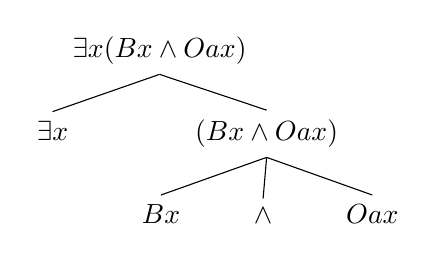
\begin{tikzpicture}[sibling distance=20pt, level distance=30pt]
    \Tree [.{$\exists x \myts (Bx \wedge Oax)$} [. $\exists x$ ] [. {$(Bx \wedge Oax)$} [. $Bx$ ] [. $\wedge$ ] [. $Oax$ ] ] ]
  \end{tikzpicture}
  \hfill
    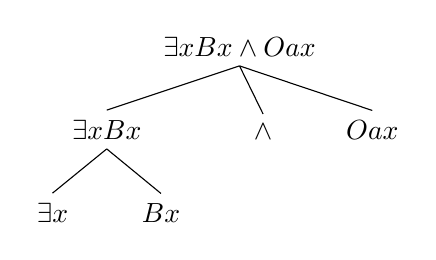
\begin{tikzpicture}[sibling distance=20pt, level distance=30pt]
    \Tree [.{$\exists x \myts Bx \wedge Oax$} [. {$\exists x \myts Bx$} [. $\exists x$ ] [. $Bx$ ] ] [. {$\wedge$} ] [. $Oax$ ] ]
  \end{tikzpicture}
\end{center}

\subsection{Terminology}

Just like in \proplog, formulas of \predlog can be named by their main operator.
For example, the following formulas can be called \emph{conjunctions}:\sidenote{The second example here expresses the idea that Alex owns a book, and that Alex likes a book, where these could be the same or different books.}
\begin{align*}
  & Oam \wedge Lam && \exists x \myts (Bx \wedge Oax) \wedge \exists x \myts (Bx \wedge Lax)
\end{align*}
A formula whose main operator is a universal quantifier can be called a \emph{universal formula} or a \emph{universal statement}; a formula whose main operator is an existential quantifier can be called an \emph{existential formula} or an \emph{existential statement}.
For example, the formula $\exists x \myts (Bx \wedge Oax)$ from above is an existential statement, but the formula $\exists x \myts Bx \wedge Oax$ is a conjunction (as evidenced by the syntactic trees given above).

If $A$ is an $n$-ary predicate letter and if $t_1, \dots, t_n$ are individual constants, then $At_1 \dots t_n$ is an \markdef{atomic sentence}.
Atomic sentences are minimal truth-evaluable units of the language of \predlog, akin to the proposition letters of \proplog.

\section{Quantifier scope \& binding}

Not every well-formed formula of \predlog is interpretable.
Consider the formula $Lax$.
We might paraphrase this as ``Alex likes them/ him/ her/ it/ you/ me/ us.''
Without knowing what $x$ refers to, this formula ---though a formula of \predlog--- is not interpretable.
We therefore introduce terminology to speak about which occurrences of variables are interpretable, which are not, and how a variable that is interpretable is to be interpreted.
The relevant technical terms are \emph{scope}, as well as \emph{bound} and \emph{free} occurrences of a variable.

If $\forall x \myts \psi$ is a subformula of $\varphi$, then $\psi$ is the \emph{scope} of this occurrence of the quantifier $\forall x$ in $\varphi$. The same holds for $\exists x$.
An occurrence of a variable $x$ in a formula $\varphi$ (in a place where also an individual constant could appear, so not the $x$ in ``$\forall x$'' and ``$\exists x$''), is \emph{free} in $\varphi$ if $x$ is not in the scope of a quantifier $\forall x$ or $\exists x$.
If $\forall x \myts \psi$ (or $\exists x \myts \psi$) is a subformula of $\varphi$ and if an occurrence of $x$ is free in $\psi$, then this occurrence of $x$ is \emph{bound} by the quantifier $\forall x$ (or $\exists x$).
A formula of predicate logic without any free occurrences of variables is called a \emph{sentence}.

Here are examples:\sidenote{The last formula is well-formed and interpretable, but not very cooperative for an interpreter. In practice, we would rather like to write $\exists x (\myts Px \wedge \forall y \myts Qy)$}
\begin{align*}
  & Px && \text{$x$ is free} \\
  & Px \wedge \forall x \myts Qx && \text{the first occurrence of $x$ is free, the second bound} \\
  & \exists x (\myts Px \wedge Qx) && \text{both occurrences of $x$ are existentially bound}\\
  & \exists x \myts Px \wedge \forall x \myts Qx && \text{first occur.~existentially bound, second universally bound}\\
  & \exists x (\myts Px \wedge \forall \myts x Qx) && \text{first occur.~existentially bound, second universally bound}
\end{align*}

\section{Domain of quantification}

Even if all variables in a formula are bound, in order to be able to interpret ---even if only intuitively--- what a formula of \predlog could mean, we need information about the \emph{domain of quantification} $D$.
Take the formula $\forall x \myts (Lxa)$ with the interpretation of $a$ and $Lxy$ as before.
We might take this to mean that everybody likes Alex, or that everything on earth (including the book \emph{Moby Dick}) likes Alex.
So, when we write down a formula with quantifiers in \predlog, it will only be interpretable if we specify which individuals the quantification should range over.
We call this the \emph{domain of quantification} $D$.
Remember that you must always specify the domain of quantification $D$ in translation exercises or other applications where your formulas are supposed to be meaningfully interpretable.

\section{Translations from natural langauge to \predlog}

Just like \proplog, \predlog is useful for uncovering the logical structure of sentences.
Unlike \proplog, \predlog can lay bare the internal structure of atomic propositions and aspects of quantification.

Suppose we want to translate this sentence to predicate logic:
\begin{quote}
Alex likes Bo but if Bo likes Alex, Bo likes everybody.
\end{quote}
A formula that captures the logical structure of this sentence is:
\begin{align*}
  Lab \wedge (Lba \rightarrow \forall x \myts Lbx)
\end{align*}
Such a translation is only complete, strictly speaking, when we also explicitly state the \emph{translation key}, which defines what each individual constant and predicate letter refers to, as well as the arity of each predicate letter.
In the example at hand, the translation key would be:\sidenote{Notice that the arity of the predicate $L$ is fixed by the notation $Lxy$ and that it is crucial for the translation key to specify exactly what a predicate like $L$ means, i.e., is first argument the slot for the person doing or receiving the liking?}
\begin{enumerate}[(i)]
  \item $a$: Alex
  \item $b$: Bo
  \item $Lxy$: $x$ likes $y$
\end{enumerate}
Since the sentence to translate includes the word ``everybody,'' the domain of quantification should be the set of all human beings for the above formula to be correct.
If the domain of quantification also includes non-humans, we would have to adapt the formula like so:
\begin{align*}
  Lab \wedge (Lba \rightarrow \forall x \myts (Hx \rightarrow Lbx))
\end{align*}
and also include the predicate letter $H$ in the translation key like so:
\begin{enumerate}[(iv)]
  \item $Hx$: $x$ is a human being
\end{enumerate}

Let us consider a few examples.
The domain of quantification $D$ is the set of all human beings.
\begin{multicols}{2}
  \begin{enumerate}
    \item[] $a$: Alex
    \item[] $b$: Bo
    \item[] $Fx$: $x$ is friendly
    \item[] $Lxy$: $x$ likes $y$
    \item[] $Px$: $x$ is a pilot
    \item[] $Sxy$: $x$ and $y$ are siblings
  \end{enumerate}
\end{multicols}
Here is a list with  sentences and potential translations into \predlog.\sidenote{For some sentences, more than one translation is given. These alternatives are logically equivalent under the semantics of \predlog which we will introduce later.}
\begin{align*}
  & \text{Alex is a pilot.}
  && Pa
  \\
  & \text{Bo is a friendly pilot.}
  && Fb \wedge Pb
  \\
  & \text{No pilot is friendly.}
  && \forall x \myts (Px \rightarrow \neg Fx)
  \\
  &&& \neg \exists x \myts (Px \wedge Fx)
  \\
  & \text{Nobody likes pilots.}
  && \neg \exists x \myts \exists y \myts (Py \wedge Lxy)
  \\
  & \text{Bo has a friendly sibling.}
  && \exists x \myts (Fx \wedge Sbx)
  \\
  & \text{Every pilot has a friendly sibling.}
  && \forall x \myts (Px \rightarrow (\exists y \myts (Fy \wedge Sxy)))
  \\
  &&& \forall x \myts \exists y \myts (Px \rightarrow (Fy \wedge Sxy)) \\
  &&& \neg \exists x \myts (Px \wedge \neg \exists y \myts (Fy \wedge Sxy)) \\
  &&& \neg \exists x \myts \neg \exists y \myts (Px \rightarrow (Fy \wedge Sxy)) \\
\end{align*}


\bigskip
\noindent \colorbox{mygray}{\centering
  \begin{minipage}{1.0\textwidth}

    \begin{exercise}
      For each of the following strings, determine whether they are formulas of \predlog or not. Assume that $P$ and $Q$ are unary predicate letters, and that $R$ is a binary predicate letter.
      \begin{multicols}{2}
      \begin{enumerate}[(i)]
        \item $Px \rightarrow \exists \myts x$
        \item $\forall x (Px)$
        \item $\forall x Px$
        \item $(\forall x Px)$
        \item $Px \vee \exists \myts x Px$
        \item $\forall y Px \vee \exists \myts x Px$
        \item $\forall y (Rxy \vee \exists \myts x Px)$
        \item $\forall y (Rxy \vee \exists \myts x Px)$
      \end{enumerate}
    \end{multicols}
    \end{exercise}

    \begin{exercise}
      For each of the following formulas of predicate logic, determine whether each occurrence of a variable is a free or bound occurrence. If it is a bound occurrence, determine which quantifier binds it.
      \begin{multicols}{2}
      \begin{enumerate}[(i)]
        \item $Px$
        \item $\exists x \myts Lxj$
        \item $\exists x \myts Lxy$
        \item $\exists x \myts Px \wedge Lxj$
        \item $\exists x \myts (Px \wedge Lxj)$
        \item $\exists x \myts (Px \wedge \forall x \myts Lxj)$
      \end{enumerate}
    \end{multicols}
    \end{exercise}

    \begin{exercise}
      Translate the following sentences into the language of predicate logic. Preserve as much of   the logical structure as possible and give the translation key and the domain of   quantification (here: $D: \text{people}$).
      \begin{enumerate}[(i)]
        \item Everybody is friendly.
        \item Everybody loves somebody.
        \item Every pilot loves Bill.
        \item If Mary is a pilot, someone loves her.
        \item Every pilot is unfriendly.
        \item Some pilots are friendly.
        \item No pilot is friendly.
        \item Nobody loves anyone who is in love with a pilot.
      \end{enumerate}
    \end{exercise}
  \end{minipage}
}

\newpage

\section{Semantics of predicate logic}
\label{sec:semant-pred-logic}

The semantics of propositional logic was formulated in terms of valuation functions, which mapped each formula to a truth value, true or false.
We thought of these as possible worlds, or possible states the world could be in.
The semantics of \predlog is slightly more complicated because in order to say which formulas are true or false, we need to interpret not just atomic propositions, but their internal structure, so to speak; we need to interpret all terms (individual constants and variables) and the predicate letters.
This is done in a so-called \emph{model}, which can similarly be thought of as a possible world.
Given a model, we can derive a valuation function.
The model fixes the domain (which individuals are there) and the meaning of the basic vocabulary of our language, i.e., the meaning of all individual constants and all predicate letters.

\subsection{Model, domain \& interpretation function}
\label{sec:model}

A \emph{model} $M = \tuple{D,I}$ for language $\mathfrak{L}$ consists of:
\begin{multicols}{2}
  \begin{itemize}
    \item[] a \emph{domain} $D \neq \emptyset$, and
    \item[] an \emph{interpretation function} $I$.
  \end{itemize}
\end{multicols}
\noindent The domain $D$ is a set of entities.\sidenote{We will always assume that the domain has at least one element.}
The interpretation function $I$ maps each element of $C$ (the set of constants of language $\mathfrak{L}$) and $\mathcal{P}$ (the set of all predicate letters of $\mathfrak{L}$) to a suitable relation on $D$:
\begin{itemize}
  \item[] if $c$ is an individual constant, then $I(c) \in D$, and
  \item[] if $P$ is an $n$-ary predicate letter, then $I(P) \subseteq D^n$.\sidenote{$D^n$ is the set of all $n$-tuples with elements from $D$.}
\end{itemize}
The interpretation $I(c)$ of a constant $c$ is the entity in the domain that $c$ stands for (e.g., its name or identifier).
The interpretation $I(P)$ of an $n$-ary predicate letter, is the set of all $n$-tuples which stand in the relation $P$ to each other.
For example, if $R$ is the one-place predicate letter denoting the property ``red,'' then $I(R)$ is the set of all red things (in the possible world we are modeling with the help of $I$).
Or, if $L$ is the two-place predicate letter denoting the relation ``$x$ likes $y$,'' then $I(L)$ is the set of all pairs of elements from the domain, e.g., $\tuple{d_{1}, d_{2}}$, such that the first likes the second (in the possible world we are modeling with the help of $I$).

\subsection{Assignment functions}
\label{sec:assignments--term}

A model $M = \tuple{D,I}$ interprets individual constants and predicate letters.
But we also need a way to assign meaning to variables.
This needs to take quantifier binding into account.
For this purpose we can use assignment functions.
Assignment functions and the interpretation function together allow us to interpret all terms (variables and individual constants).

An \emph{assignment function} $g$ for model $M = \tuple{D,I}$ and language $\mathfrak{L}$ maps all variables in $\mathfrak{L}$ to elements in $D$.
We write $g_{[x/d]}$ and read ``$g$ with $x$ mapped to $d$'', for the assignment function which is like $g$ except that $x$ is mapped to $d \in D$.
We will use this latter construct, $g_{[x/d]}$ to define the semantics of existential and universal formulas (see below).\sidenote{If needed, this notation can also be extended to cover more than one variable, like so: $g_{[x/d_{1}, y/d_{2}, z/d_{3}]}$.}

If $t$ is a term of $\mathfrak{L}$, then $\den{t}_{M,g}$ is the \emph{term interpretation} relative to $M = \tuple{D,I}$ and $g$:
\begin{multicols}{2}
  \begin{itemize}
    \item[] $\den{t}_{M,g} = I(t)$ if $t$ is a constant, and
    \item[] $\den{t}_{M,g} = g(t)$ otherwise.
  \end{itemize}
\end{multicols}

\subsection{Valuation functions}
\label{sec:valuation--truth}

We now can use a model $M = \tuple{D, I}$ and an assignment function $g$ to define a valuation function $V_{M,g}$, which uses $M$ and $g$, to give a truth value for every formula of predicate logic.
Here is the full definition, which we will go through systematically below.

\medskip

\begin{tabular}{lcl}
  $V_{M,g}(At_1\dots t_n) =1$ & iff & $\tuple{\den{t_1}_{M,g}, \dots, \den{t_1}_{M,g}} \in I(A)$\\
  $V_{M,g}(\neg \phi) = 1$ & iff & $V_{M,g}(\phi) =0$\\
  $V_{M,g}(\phi \wedge \psi) = 1$ & iff & $V_{M,g}(\phi) =1$ and $V_{M,g}(\psi) = 1$\\
  $V_{M,g}(\phi \vee \psi) = 1$ & iff & $V_{M,g}(\phi) =1$ or $V_{M,g}(\psi) = 1$\\
  $V_{M,g}(\phi \rightarrow \psi) = 0$ & iff & $V_{M,g}(\phi) =1$ and $V_{M,g}(\psi) = 0$\\
  $V_{M,g}(\phi \leftrightarrow \psi) = 1$ & iff & $V_{M,g}(\phi) = V_{M,g}(\psi)$\\
  $V_{M,g}(\forall x \myts \phi) = 1$ & iff & $V_{M,g_{[x/d]}}(\phi) = 1$ for all $d \in D$\\
  $V_{M,g}(\exists x \myts \phi) = 1$ & iff & $V_{M,g_{[x/d]}}(\phi) = 1$ for at least one $d \in D$
\end{tabular}

\medskip

For the most basic kind of formula, built from an $n$-ary predicate letter $A$ with $n$ terms $t_{1}, \dots, t_{n}$ (where each $t_{i}$ is either a variable or an individual constant), the formula $At_1\dots t_n$ is true, given $M = \tuple{D, I}$ and $g$, if the $n$-tuple of entities picked out by the interpretation of all terms, using $I$ and $g$, is contained in the interpretation of $A$.

\medskip

\begin{tabular}{lcl}
  $V_{M,g}(At_1\dots t_n) =1$ & iff & $\tuple{\den{t_1}_{M,g}, \dots, \den{t_n}_{M,g}} \in I(A)$
\end{tabular}

\medskip

For sentential connectives, valuation functions work exactly like in \proplog.

\medskip

\begin{tabular}{lcl}
  $V_{M,g}(\neg \phi) = 1$ & iff & $V_{M,g}(\phi) =0$\\
  $V_{M,g}(\phi \wedge \psi) = 1$ & iff & $V_{M,g}(\phi) =1$ and $V_{M,g}(\psi) = 1$\\
  $V_{M,g}(\phi \vee \psi) = 1$ & iff & $V_{M,g}(\phi) =1$ or $V_{M,g}(\psi) = 1$\\
  $V_{M,g}(\phi \rightarrow \psi) = 0$ & iff & $V_{M,g}(\phi) =1$ and $V_{M,g}(\psi) = 0$\\
  $V_{M,g}(\phi \leftrightarrow \psi) = 1$ & iff & $V_{M,g}(\phi) = V_{M,g}(\psi)$
\end{tabular}

\medskip

Finally, to assign a truth-value to existential or universal formulas, we use the construction $g_{[x/d]}$, which represents an assignment function which is exactly like $g$ but with a special, possibly different interpretation for the variable $x$.

\medskip

\begin{tabular}{lcl}
  $V_{M,g}(\forall x \myts \phi) = 1$ & iff & $V_{M,g_{[x/d]}}(\phi) = 1$ for all $d \in D$\\
  $V_{M,g}(\exists x \myts \phi) = 1$ & iff & $V_{M,g_{[x/d]}}(\phi) = 1$ for at least one $d \in D$
\end{tabular}

\section{Truth in a model}

Assignment functions are just auxiliary constructs.
At the end of the day, we are interested in whether a formula is true in a possible world, i.e., a model $M = \tuple{D,I}$, no matter what assignment function is used.

If $V_{M,g}(\varphi) = 1$ for all $g$, we write $V_{M}(\varphi) = 1$ and say ``$\varphi$ is true in $M$.''
If $V_{M,g}(\varphi) = 0$ for all $g$, we write $V_{M}(\varphi) = 0$ and say ``$\varphi$ is false in $M$.''

Notice that any \emph{sentence} of \predlog (i.e., any formula without free variables) is either true or false in any given model $M$.
In other words, formulas without free occurrences of variables are interpretable just with respect to a model, and these formulas are ---usually--- what we care about.

Let's consider a simple example of a model and the way it makes certain sentences true or false.
The language we are interested in has just one individual constant $a$, two one-place predicate letters, $P$ and $Q$, as well as one two-place predicate letter $R$.
An example model $M = \tuple{D, I}$ for this language, fixing a domain and an interpretation of all basic vocabulary, can be written out like this:
\begin{align*}
  D    & = \set{1,2,3,4,5}\\
  I(a) & = 3 \\
  I(P) & = \set{1,2,5} \\
  I(Q) & = \set{2,5} \\
  I(R) & = \set{\tuple{1,2},\tuple{2,2}, \tuple{1,4}, \tuple{1,5}}
\end{align*}

For better visual grasp, small models can often be represented economically as a graph.
Figure~\ref{fig:predlog-exmple-model} is an example for the model at hand.
The two-place relation is represented in terms of arrows, small letters ornamenting the elements of the domain show the interpretation of individual constants and one-place predicate letters.

\begin{figure}
  \centering
  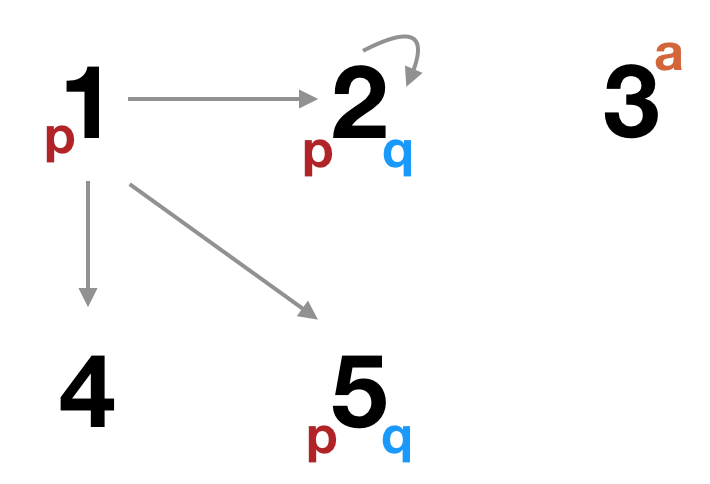
\includegraphics[width=0.5\textwidth]{00-pics/predlog-example-model.png}
  \caption{Example of a graphical representation of a simple model for predicate logic.}
  \label{fig:predlog-exmple-model}
\end{figure}

A graphical representation like in Figure~\ref{fig:predlog-exmple-model} greatly facilitates checking whether a model makes certain sentences true or false.
For example, in order to decide whether a formula like $\exists x \myts (Px \wedge Qx)$ is true or false in this model, we need to check whether there is an element that has both property $P$ and property $Q$.
Looking at Figure~\ref{fig:predlog-exmple-model}, we see that this is true.
Elements 2 and 5 both have both properties.
To write this down in a formally correct way with reference to the model's mathematical structure and the definition of the semantics of \predlog, we would say that $V_{M}(\exists x \myts (Px \wedge Qx)) = 1$ because, no matter which $g$ we use, there exists an element in $D$, namely 2, such that $V_{M,g[x/2]}(Px \wedge Qx) = 1$. This is because $2 \in I(P)$ and $2 \in I(Q)$.

Take another example.
What is the truth value that the model assigns to formula $Pa$?
Well, that formula is false in the given model.
The individual referred to by constant $a$ is 3, but 3 does not have property $P$.
In formal terms, we would then say that $V_{M}(Pa) = 0$, because, for any valuation function $g$, since $I(a) = 3$ and $3 \not \in I(P)$, we have $V_{M,g}(P(a)) = 0$.



\section{Validity}
\label{sec:validity}

Validity is defined in the same way in \predlog as it was in \proplog.

If $\varphi_1, \dots, \varphi_n$ and $\psi$ are sentences of predicate logic, $\varphi_1, \dots, \varphi_n / \psi$ is an \emph{argument schema}.
The argument schema $\varphi_1, \varphi_2, \dots, \varphi_n / \psi$ is \emph{valid} iff for all models $M$ such that $V_M(\varphi_1)=V_M(\varphi_2)= \dots = V_M(\varphi_n)=1$ it also holds that $V_M(\psi) = 1$.
If valid, we write $\varphi_1, \varphi_2, \dots, \varphi_n \models \psi$.

In order to demonstrate that an argument schema is not valid, it suffices to give a single counterexample.
In order to demonstrate that a given argument schema is valid, we need to give an informal proof, since we must reason over \emph{all} models. %\sidenote{Notice that the later, demonstrating validity with an informal proof, is much more difficult and should be consider as a skill that is not necessary to pass an introductory logic course, but one that is only required for an excellent grade.}
The following gives examples for each.


\subsection{Demonstrating invalidity with a counterexample}
\label{sec:demonstr-inval-with}

\begin{claim}
 $\exists x \myts Px  \not \models \ \forall x \myts Px$\sidenote{Intuitively, just because someone is a pilot, doesn't mean that everybody is a pilot.}
\end{claim}
\begin{proof}
A minimal counterexample for this case is a model $M$ with domain $D = \set{1,2}$ and interpretation function $I(P) = \set{1}$.
It is clear that there is an element $d \in D$, namely 1, such that $V_{M,g[x/1]}(Px)$ is true, so that the premise $\exists x \myts Px$ is true in $M$.
But there is also an element $d \in D$, namely 2, such that $V_{M, g[x/2]} Px$ is false, so that the conclusion $\forall x \myts Px$ is false in $M$.
\end{proof}

\subsection{Demonstrating validity with an informal proof}
\label{sec:demonstr-valid-with}

Here are two examples for informal proofs demonstrating validity of an argument schema.

\begin{claim}
  $\forall x \myts Px \ \models \ \neg \exists x \myts \neg Px$\sidenote{Intuitively, if everybody is a pilot, there cannot be anyone who is not a pilot.}
\end{claim}

\begin{proof}
  We need to show that for all models $M$, if $V_{M}(\forall x \myts Px) = 1$, then $V_{M}(\neg \exists x \myts \neg Px) = 1$.
  So suppose that we have an arbitrary model $M = \tuple{D,I}$, such that $V_{M}(\forall x \myts Px) = 1$.
  This entails that for all $d \in D$, $d \in I(P)$.
  Suppose further, towards contradiction, using an indirect proof strategy, that for the same $M$ we have $V_{M}(\neg \exists x \myts \neg Px) = 0$.
  The latter means that $V_{M}(\exists x \myts \neg Px) = 1$, which is the case when there is an element $d \in D$ such that $d \not \in I(P)$.
  But that contradicts the inference we drew from our premise that for all $d \in D$, $d \in I(P)$.
  Consequently, there cannot be a model $M$ which makes the premise true and the conclusion false.
  The argument schema must be valid.
\end{proof}

\begin{claim}
  $\neg \forall x \ (Px \rightarrow Fx) \models \exists x \ Px$\sidenote{Intuitively, if it is not the case that every pilot is friendly, there has to be at least one pilot.}
\end{claim}

\begin{proof}
  Assume that the premise $\neg \forall x \ (Px \rightarrow Fx)$ is true in a model $M = \langle D, I \rangle$.
  From $V_M(\neg \forall x \ (Px \rightarrow Fx))=1$ we know that $V_M(\forall x \ (Px \rightarrow Fx))=0$.
  But if $\forall x \ (Px \rightarrow Fx)$ is false in $M$, it follows that there is at least
  one element $d \in D$ such that $V_{M, g_{[x/d]}} (Px \rightarrow Fx) = 0$, for arbitrary $g$.
  We know that an implication is only false if the antecedent is true and the consequent is false (from propositional logic, definition of $\rightarrow$).
  That means that it must be the case that $V_{M, g_{[x/d]}}( Px ) = 1$.
  This entails that $V_{M, g} (\exists x \myts Px)=1$, by definition of truth of existential statements.
  But since $g$ was completely arbitrary and nothing hinges on any specifics of $g$, we have actually shown that $V_M(\exists x \ Px) =1$.
\end{proof}

\section{Equivalences, tautologies and contradictions}
\label{sec:equivl-taut-contr}

The notions of \emph{logical equivalence}, \emph{tautology} and \emph{contradiction} for \predlog are all analogous to their counterparts in \proplog.

Two formulas $\varphi$ and $\psi$ of \predlog are logically equivalent iff for all models $M$ we have $V_{M}(\varphi) = V_{M}(\psi)$. A formula $\varphi$ of \predlog is a tautology iff for all models $M$ we have $V_{M}(\varphi)=1$. It is a contradiction iff for all models $M$ we have $V_{M}(\varphi)=0$.

In order to demonstrate that two formulas are logically equivalent, or that a formula is a tautology or contradiction, we can give informal proofs. For example, the previous section showed that $\forall x \myts Px \ \models \ \neg \exists x \myts \neg Px$. In fact, $\forall x \myts Px$ and $\neg \exists x \myts \neg Px$ are logically equivalent. Here is an informal proof for this:

\begin{claim}
  \label{claim:equivalence-universal-existential}
  $\forall x \myts Px$ and $\neg \exists x \myts \neg Px$ are logically equivalent.
\end{claim}

\begin{proof}
  Let $M$ be a model in which $\neg \exists x \myts \neg Px$ is true.
  This means that there is not a single element $d \in D$, such that $d \not \in I(P)$.
  In other words, $I(P) = D$, i.e., all elements in the domain have property $P$.
  So $M$ also makes $\forall x \myts Px$ true.
  The reverse direction has already been shown when proving $\forall x \myts Px \ \models \ \neg \exists x \myts \neg Px$.
\end{proof}

\newpage

\bigskip
\noindent \colorbox{mygray}{\centering
  \begin{minipage}{1.0\textwidth}

    \begin{exercise}
      Use the model from the example in Figure~\ref{fig:predlog-exmple-model} to check the truth value of the following formulas.
      \begin{multicols}{2}
        \begin{enumerate}
          \item $\neg Qa$
          \item $\forall x \ (Qx \rightarrow Px)$
          \item $\neg \exists x \ Rxx$
          \item $\exists x \exists y \ (Qx \wedge Py \wedge Rxy)$
          \item $\forall x \exists  y \ Rxy$
          \item $\forall x \forall y \ (Rxy \rightarrow (Px \vee Qy))$
        \end{enumerate}
      \end{multicols}
    \end{exercise}

    \begin{exercise}
      Consider a model $M = \tuple{D,I}$ for a language with two unary predicate letters $P$ and $Q$ and a two-place predicate letter $R$, given as follows.
      \begin{align*}
        D    & = \set{1,2,3,4,5}\\
        I(P) & = \set{1,2,5} \\
        I(Q) & = \set{2,5} \\
        I(R) & = \set{\tuple{1,2},\tuple{2,2}, \tuple{1,4}, \tuple{1,5}}
      \end{align*}
      Evaluate for each of the following formulas whether they are true or false in the model.
      (Hint: It is highly recommended that you draw a graphical representation for yourself similar to Figure~\ref{fig:predlog-exmple-model}, even if that is not required to obtain points and/or a correct solution.)
      \begin{multicols}{2}
        \begin{enumerate}
          \item $\exists x \ (Px \wedge Qx)$
          \item $\forall x \ (Qx \rightarrow Px)$
          \item $\neg \exists x \ Rxx$
          \item $\exists x \exists y \ (Qx \wedge Py \wedge Rxy)$
          \item $\forall x \exists  y \ Rxy$
          \item $\forall x \forall y \ (Rxy \rightarrow (Px \vee Qy))$
        \end{enumerate}
    \end{multicols}
    \end{exercise}

    \begin{exercise}
      Give informal proofs or counterexamples for these claims:
        \begin{enumerate}[(i)]
          \item $\forall x \ (Ax \vee Bx \vee Cx), \ \ \forall x \ (Ax \rightarrow Bx), \ \ \neg \exists Bx \models \exists x \ Cx$
          \item $\exists x \, Ax, \ \exists x \, Bx \models \exists x \, (Ax \wedge Bx)$
          \item $\forall x \forall y \forall z \ ((Rxy \wedge Ryz) \rightarrow
          Rxz), \ \ \exists x \exists y \ (x \neq y \wedge Rxy \wedge Ryx) \
          \ / \ \ \exists x \ Rxx$
          \item $\forall x \, (Ax \vee Bx) \models \forall x \, Ax \vee \forall x \, Bx$
          \item $\forall x \ (Ax \leftrightarrow Rxx), \ \exists x \forall y \
          (Ryy \leftrightarrow x=y) \models \exists x \ Ax$
          \item $\exists x \forall y \ Rxy, \ \forall x \forall y \ (Rxy
          \rightarrow Ryx) \models \forall x \ \exists y \ Rxy$
          \item $\forall x \, (Ax \rightarrow Bx),  \exists x \, Bx \models  \neg \exists x \, Ax$
        \end{enumerate}

    \end{exercise}

  \end{minipage}
}

\newpage

\section{Predicate logic with identity}
\label{sec:predicate-logic-with}

Suppose we want to translate the meaning of the following sentence into predicate logic:
\begin{quote}
  Only Alex is a pilot.
\end{quote}
We can write $Pa$ (with the obvious translation key), expressing that Alex is a pilot.
But we also want to express that nobody else is.
We can express that nobody is a pilot with a formula like $\forall x \myts \neg Px$ or, equivalently (see Claim~\ref{claim:equivalence-universal-existential}), $\neg \exists \myts Px$.
But that's not actually true because Alex is.
So writing $Pa \wedge \forall x \myts \neg Px$ is a contradiction that does not express the meaning of ``Only Alex is a pilot.''
Indeed, \predlog as we defined it so far is not expressive enough to capture the meaning of this sentence.
We need to add something.
We will add a special predicate: identity.

\subsection{Adding identity to \predlog}

We change clause (i) of the definition of formulas of predicate logic, given in Section~\ref{sec:formulas}, to also allow the use the special two-place predicate symbols ``='' and ``$\neq$'' for which we use infix notation.

\begin{enumerate}[(i)]
  \item If $A$ is an $n$-ary predicate letter and if $t_1, \dots, t_n$ are terms, then $At_1 \dots t_n$ is a formula. \textbf{If $t_1$ and $t_2$ are terms, then $t_1 = t_2$ and $t_1 \neq t_2$ are formulas.}
\end{enumerate}

These are special symbols also in the semantics, because they are interpreted in the same manner in every model.\sidenote{
  Identity is the same concept in all possible worlds.
  It is a logical concept that has a fixed meaning in all (logically) possible worlds.
}
Concretely, we just add the following clause to the definition of the semantics of predicate logic:\sidenote{
  Notice that there are three occurrences of the symbol ``='' in the first line of this definition.
  The first occurrence refers to the two-place predicate letter of \predlog with identity.
  The latter two refer to our usual understanding of ``='' as identity.
  Basically, this is a complicated way of saying that ``='' is supposed to mean the same same thing in \predlog as what it means outside of it.
}

\medskip

\begin{tabular}{lcl}
  $V_{M,g}(t_1 = t_1) = 1$ & iff & $\den{t_1} = \den{t_{2}}$ \\
  $V_{M,g}(t_1 \neq t_1) = 1$ & iff & $\den{t_1} \neq \den{t_{2}}$
\end{tabular}

\medskip

\subsection{Translations with \predlog with identity}

Using identity in the logical language, we can express the meaning of
\begin{quote}
  Only Alex is a pilot.
\end{quote}
in terms of the formula:
\begin{align*}
  Pa \wedge \forall x \myts (x \neq a \rightarrow \neg Px)
\end{align*}
which can be read as: ``Alex is a pilot, and everybody who is not Alex is not a pilot.''\sidenote{This is not the only paraphrase and formula we can give to this example. See the first example in the list that follows, for instance.}

Here are further examples for translations, making use of identity:\sidenote{Translation key as before.}

\begin{enumerate}[(i)]
  \item Alex is friendly but nobody else is.
  \hfill {\mygray{$Fa \wedge \forall x \, (Fx \rightarrow x = a)$}}
  \item At least two people are friendly.
  \hfill {\mygray{$\exists x \exists y \, (Fx \wedge Fy \wedge x \neq y)$}}\sidenote{
    We omit parentheses here, even though they would be strictly speaking required by the definition of a formula.
    Instead of writing $\varphi \wedge (\psi \wedge \chi)$ or $(\varphi \wedge \psi) \wedge \chi$, given that these two formulas are logically equivalent (in \proplog and in \predlog), we simply write $\varphi \wedge \psi \wedge \chi$.
  }
  \item Alex likes only pilots, except for Bo.
  \hfill {\mygray{$\forall x \, (Lax \rightarrow (Px \vee x = b))$}}
  \item Exactly two people are pilots.\\
  \hfill {\mygray{$\exists x \exists y \, (x \neq y \wedge
  Px \wedge Py \wedge \forall z \, (Pz \rightarrow (z = x \vee z = y)))$}}
  \item Bo likes at most two people. \\
  \hfill {\mygray{$\forall x \forall y \, (((Lbx \wedge Lby) \wedge x \neq y) \rightarrow \forall z \,
  (Lbz \rightarrow (z = x \vee z = y)))$}}
\end{enumerate}

\subsection{Translating modified numerals}
\label{sec:transl-modif-numer}

Translations of quantified expressions like ``at most two people,'' as in the last example, can be difficult.
For example, ask yourself: Is the following translation adequate for the last example of ``Bo likes at most two people?''
\begin{enumerate}[(v)]
  \item Bo likes at most two people. \\
  \hfill {\mygray{$\forall x \forall y \, ((Lbx \wedge Lby)
  \rightarrow \forall z \, (Lbz \rightarrow (z = x \vee z = y)))$}}
\end{enumerate}
No it is not.
This is because that last formula is false in a world in which Bo loves two people.
Suppose Bo loves Alex and Charley, and that Alex, Bo and Charley are three different people.
Let $x$ and $y$ refer to Alex.
Then the antecedent $(Lbx \wedge Lby)$ becomes true.
Let $z$ refer to Charley.
Bo loves Charley, but Charley is not identical to Alex (by assumption).

Expressions like ``at most two'' or ``exactly one'' are called \emph{modified numerals}.
Here are some templates for translating these kinds of expressions into predicate logic with identity.
The following are example translations for modified numerals applied to a unary predicate $P$.
\begin{align*}
  \text{at least one} &&& \exists x \myts Px \\
  \text{at least two} &&& \exists x \myts  \exists y \myts (Px \wedge Py \wedge x \neq y) \\
  \text{exactly one}  &&& \exists x \myts (Px \wedge \forall y \myts (Py \rightarrow x = y) )\\
  \text{exactly two}  &&& \exists x \myts \exists y \myts (x \neq y \wedge Px \times Py \wedge \forall z \myts (Pz \rightarrow (z = x \vee z = y))) \\
  \text{at most one}  &&& \forall x \myts \forall y \myts ((Px \wedge Py) \rightarrow x = y) \\
  \text{at most two}  &&& \forall x \myts \forall y \myts ((Px \wedge Py \wedge x \neq y) \rightarrow \forall z \myts (Pz \rightarrow (z =x \vee z = y)) )
\end{align*}


\bigskip
\noindent \colorbox{mygray}{\centering
  \begin{minipage}{1.0\textwidth}

    \begin{exercise}
      Translate the following sentences into predicate logic with identity.
      \begin{enumerate}[(i)]
        \item Only Alex and Bo are friendly.
        \item If Alex is friendly, nobody else is.
        \item Alex is the only friendly pilot.
        \item There is a pilot but it is not Alex.
        \item There is at most one pilot.
        \item Alex likes nobody but Bo and Alex.
      \end{enumerate}
    \end{exercise}

  \end{minipage}
}




\end{document}
